\section {Image recognition}
Image recognition is a very interesting topic in computer vision and pattern recognition, and the goal is to recognize different classes in images. For instance, there are trees, people, sun, moon and buildings in different images. Human can easily distinguish different classes among a set of images. However, machines are not good at such tasks. For many years, a lot of researchers are working on this topic and have achieved significant results.\\

\noindent So far, a very good framework to recognize images is the so-called {\em bag of words} model, which generalizes from natural language processing (NLP). In NLP, bag of words basically aims to represent an article using histogram of word frequencies. Following this idea, in image recognition, an image is also represented as a histogram of visual words, and these visual words normally come from centroids generated from clustering algorithms. Later on, such representations of images are used to build up generic machine learning models, and the accuracy is quite impressive. During recognition phase, the most critical process is to calculate image-to-image distance. One direct way is the Euclidean distance. But a better way to calculate distance is called as Earth Mover's Distance \cite{rubner2000earth}, which finds the best matches between image parts and produces a more accurate distance.

\noindent In the following of this section, an image recognition framework consisting of 4 steps is first introduced. Secondly, Earth Mover's distance and its applications in image recognition is talked about. Lastly, the method to identify duplicates in a cluster of images used in this project are presented, and this method is going to be applied in video recognition to show the effectiveness of Earth Mover's distance.

\subsection{Framework description}

Generally, there are 4 below steps to go:

\subsubsection{Extract SIFT features from each image}
It is almost impossible to directly rely on pixel data of images to perform recognition tasks, and the main reason is because such pixel data does not possess much discriminative power. Therefore, other approaches to represent images are needed. One approach is to extract features from images and use those features to represent images compactly. There are generally two categories of features: global features and local features.

Features play an important role in recognition systems.


\begin{enumerate}
	\item {\bfseries Extract SIFT features from each image}
	\\SIFT is short for scale-invariant feature transform introduced by David G. Lowe in 1999 \cite{lowe1999object}. Given SIFT's ability to find distinctive key points that are invariant to location, scale and rotation, it is very robust to be used for image recognition. Here for simplicity, an open source library VLFEAT \cite{vedaldi08vlfeat} is adopted to extract this feature from images. The dense SIFT feature is extracted at path size 16 with step to be 8, and the number of dimension for each feature is 128.

	\item {\bfseries Build up visual vocabulary from features of training set}
  \\Similar to natural language processing, a vocabulary is needed to represent images. Commonly, K-means algorithm is performed on features resulting from training set, and the final centroids are treated as words of vocabulary. In this experiment, there are 157920 SIFT features extracted from training images. Due to this large number, MiniBatchKMeans \cite{sculley2010web}, a variant of KMeans algorithm which uses min-batches to reduce the computation time in library scikit-learn \cite{scikit-learn}, is used to generate a vocabulary, and the number of centroids is set to be 300. Thus, the vocabulary size is 300.

	\item {\bfseries Construct a pyramid of three levels for each image}
  \\The pyramid match kernel is introduced by Kristen Grauman and Trevor Darrell \cite{grauman2005pyramid} in 2005. In this method, a pyramid is built for each image level by level through increasing histogram resolution. However, this method ignores spatial information among images. After one year, spatial pyramid matching is introduced \cite{lazebnik2006beyond}. Like the name has stated, pyramid is built by taking spatial information into consideration. There are three levels built: level 0 takes the whole image as input and produce a single histogram; level 1 divides an image into 4 parts equally and produces 4 histogram in total; level 2 divides an image into 16 parts equally and outputs 16 histograms in total. Also, the weight is decreasing with level increasing when calculating distances between images. In this experiment, the spatial pyramid matching is implemented independently without help from libraries. Since the vocabulary size is 300, the numbers of dimension are 300, 1500, 6300 for $Level 1$, $(Level 1 + Level 2)$ and $(Level 1 + Level 2 + Level 3)$ respectively.

	\item {\bfseries Classify based on above representations} 
  \\Support vector machines are supervised learning models to analyze data and recognize patterns. In addition to performing linear classification, SVMs can also efficiently perform non-linear classification through kernel trick, which implicitly maps data into high dimensional feature spaces. In this experiment, LIBSVM \cite{CC01a} is used, and multi-class classification is performed in ``one-against-one'' approach. Experiments of different kernels at different levels have been conducted, and detailed analysis are presented in experiment section.
\end{enumerate}

\subsection{Earth mover's distance and its application}
According to Rubner, Tomasi and Guibas \cite{rubner2000earth}, the earth mover's distance is formulated as the following linear programming problem: Let $P = \{(p_1, w_{p1} ), . . . , (p_m , w_{pm} )\}$ be the first signature with $m$ clusters, where $p_i$ is the cluster representative and $w_{pi}$ is the weight of the cluster; $Q=\{(q1,w_{q1}),...,(qn,w_{qn})\}$ the second signature with $n$ clusters; and $D = [d_{ij}]$ the ground distance matrix where $d_{ij}$ is the ground distance between clusters $p_i$ and $q_j$. \\

\noindent We want to find a flow $F = [f_{ij}]$, with $f_{ij}$ the flow between $p_i$ and $q_j$, that minimizes the overall cost: $$WORK(P , Q, F) = \sum_{i=1}^{m}\sum_{j=1}^{n}d_{ij}f_{ij},$$ subjective to the following constraints: 
$$f_{ij} \geq 0 \quad \quad 1 \leq i \leq m,  1 \leq j \leq n $$ 
$$\sum_{j=1}^n f_{ij} \leq w_{pi} \quad 1 \leq i \leq m$$
$$\sum_{i=1}^m f_{ij} \leq w_{qj} \quad 1 \leq j \leq n$$
$$\sum_{i=1}^{m} \sum_{j=1}^n f_{ij} = min(\sum_{i=1}^m w_{pi}, \sum_{j=1}^n w_{qj})$$

\noindent Once the above linear programming problem is solved, the earth mover's distance is defined as the resulting work normalized by the total flow:
$$EMD(P, Q) = \frac{\sum_{i=1}^m \sum_{j=1}^n d_{ij} f_{ij}}{\sum_{i=1}^m\sum_{j=1}^n f_{ij}}$$

\begin{figure}[!ht]
\centering
	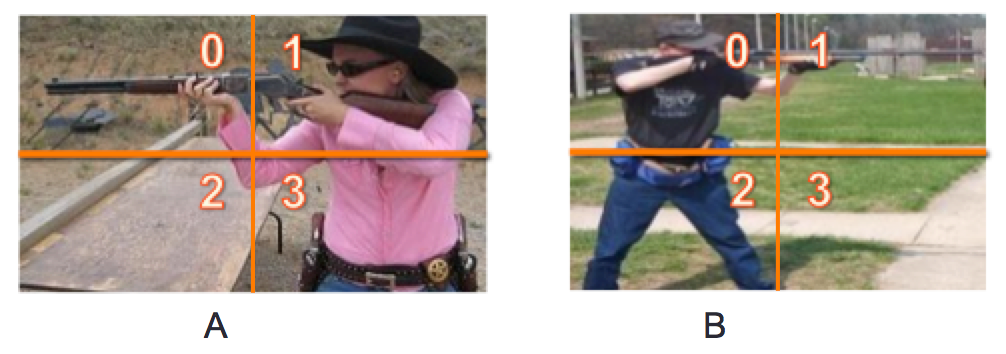
\includegraphics[width=1\textwidth]{./image_EMD_Sample.png}
\caption{Image division}
\end{figure}

\noindent Specific to calculate image distances, the first step is to divide each image into four parts equally. An example is depicted in Figure 1. There are two images $A$ and $B$, and they are both divided into 4 parts. Each part is then represented by a histogram using the vocabulary built above. As a result, such representation is identical to pyramid at level one. Afterward, image $A$ and $B$ are represented as below:
	$$A = \{(a_0, 0.25), (a_1, 0.25), (a_2, 0.25), (a_3, 0.25)\}$$
	$$B = \{(b_0, 0.25), (b_1, 0.25), (b_2, 0.25), (b_3, 0.25)\}$$
where $a_0, a_1, a_2, a_3$ and $b_0, b_1, b_2, b_3$ are respective histograms.\\

\noindent Here, the distance matrix $D$ is constructed by Euclidean distance between histograms. A sample distance matrix of the two images in Figure 1 is shown below in Table 1. 

\begin{table}[!ht]
    \begin{center}
    \scalebox{0.8}{
      \begin{tabular}{ccccc}
      \hline
      \head{} & \head{$b_0$} & \head{$b_1$} & \head{$b_2$} &\head{$b_3$} \\
    $a_0$ & 27.06473721	& 23.37733946	& 29.18047292 &	32.61901286\\
	$a_1$ & 20.84466359	& 21.50581317	& 21.70253441 &	30.34798181\\
	$a_2$ & 26.48584528	& 27.38612788	& 27.46816339 &	34.71310992\\
	$a_3$ & 19.31320792	& 24.20743687	& 21.59861107 &	31.81194744\\
      \hline
      \end{tabular}
    }
    \end{center}
    \caption{Distance matrix}
\end{table}

\noindent If there is no alignment, the distance is calculated as below:
$$d_{00} + d_{11} + d_{22} + d_{33} = 107.851$$

\noindent Once the linear programming is solved, the matches depicted in Figure 2 are found. In this case, the EMD is calculated as below:
$$d_{30} + d_{12} + d_{01} + d_{23} = 99.106$$

\begin{figure}[!ht]
\centering
	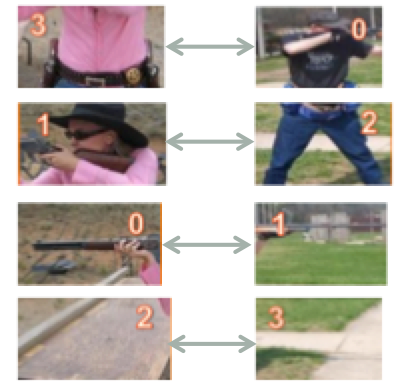
\includegraphics[scale = 0.8]{./image_EMD.png}
\caption{EMD match of images}
\end{figure}

\noindent It is easy to see that EMD is significantly smaller than the distance calculated without alignment. As Figure 2 shows, $a_0$ and $b_1$, which both represent a gun, are perfectly matched. Such example shows the effectiveness of earth mover's distance. More details about EMD's application in image recognition are presented in the experimental section.

\subsection {Key frame identification in cluster of images}
By noticing that some consecutive frames in video are similar to each other, it is thought that video can be described by several key frames. In doing so, the data to represent each video can thus be largely reduced. One key step in key frame identification is to check whether two images are near duplicate. If three images are examined to be near duplicates, only one image will be selected to represent these three images. The rest of this section will focus on two parts: near duplicate identification and how this duplicate identification is applied to identify key frames in videos.

\subsubsection{Identifying near duplicate}
Currently, the way which has been implemented to check whether two images are near duplicate follows the method stated on paper \cite{zhao2007near}. In the paper, there are basically three steps. Firstly, the authors propose to use a hash table to match SIFT points. Secondly, a SVM classifier is built based on the matching SIFT points. Finally, this classifier could be used to check near duplicates. Due to a lack of training set, the classifier is not built now, and a threshold is set to replace the classifier. It means that two images are treated as near duplicate as long as the number of matching interest point is large enough. Later on, if possible, a classifier will be built to enhance the performance. \\

\noindent In order to minimize false matches, the authors propose one-to-one symmetric matching \cite{zhao2007near}, which ensures all the matches are nearest neighbors. One the other hand, the symmetric property makes sure that the matching result of set A to B is exactly the same as B to A. Suppose there are two images $I_1$ and $I_2$, the steps to check whether these two images are near duplicate go as below:

\begin{enumerate}
  \item{\bfseries Perform PCA on SIFT features of $I_1$ and $I_2$ to reduce dimensions}
  The dimension of SIFT feature is reduced from 128 to 36, and each value of reduced feature is normalized to be within the range [0, 2]. 

  \item{\bfseries Hash all interest points of $I_1$ into a $8 \times 36$ table}

  \begin{figure}[!ht]
  \centering
    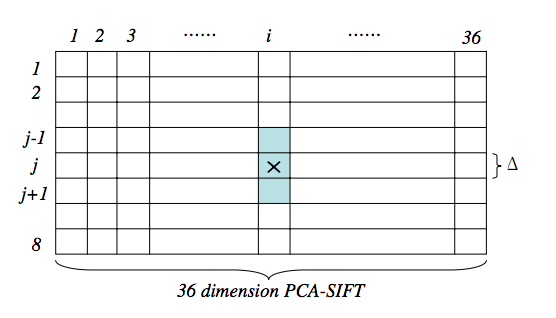
\includegraphics[scale = 0.8]{./hashTable.png}
  \caption{$8 \times 36$ Hash Table \cite{zhao2007near}}
  \end{figure}
  
  The hash table is composed of $8 \times 36$ bins as shown in Figure 3. Given each point $P = [p_1, p_2,..., p_{36}]$ of $I_1$, the index of $p_i$ is hashed to, 
  $$H(p_i) = \lfloor p_i \times 4 \rfloor$$ 
  Since the dimension is 36, $P$ is repeatedly indexed into the corresponding bin for 36 times, according to its quantized value in a particular dimension.   
  
  \item{\bfseries For each interest point $Q$ of $I_2$, examine whether there is a match in $I_1$}\\
  There are three sub steps to go:
    
    \begin{enumerate}
    \item {Hash $Q$ into the hash table}
    \item {Retrieve the set $A(Q)$ satisfying the below constraints}\\
    For each interest point $P \in I_1$, put $P$ into $A(Q)$ if $$\sum_{i=1}^{36}f(q_i, p_i) = 36$$ 

    where 
    \begin{equation*}
        f(q_i, p_i) = \begin{cases}
                   1     & \text{if } \left|H(q_i) - H(p_i)\right| \leq 1\\
                   0 & \text{otherwise}
               \end{cases}
    \end{equation*}

    \item {If $A(Q)$ is not empty, find the nearest neighbor $M \in A(Q)$ with one-to-one symmetric constraint as $Q$' match}
    \end{enumerate}

  \item{\bfseries If the number of matching interest point is large enough, $I_1$ and $I_2$ are near duplicates}
\end{enumerate}

\noindent An example of performing the above algorithm is depicted below in Figure 4. Those colored lines in the upper two images connect the matched interest points, and it is easy to distinguish that the matching accuracy is quite high because of one-to-one constraint. Please also notice that only partial matching points are drawn for better visualization. 
  \begin{figure}[!ht]
  \centering
    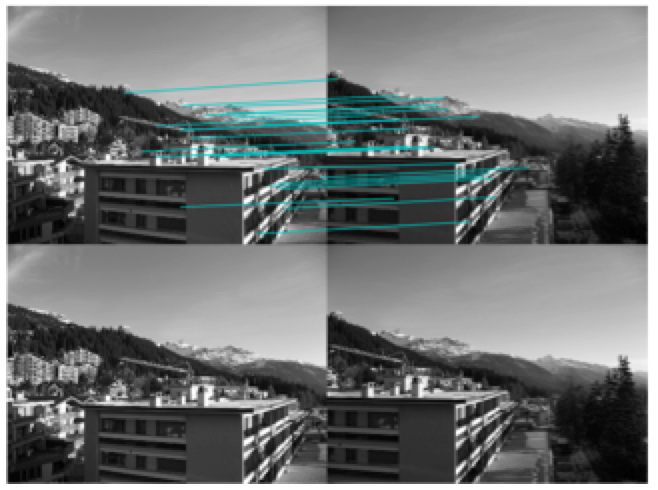
\includegraphics[scale = 0.8]{./match.png}
  \caption{Near duplicate example}
  \end{figure}

\subsubsection{Identifying key frames} 
Now that near duplicate method is introduced, it is time to check how this method is incorporated into key frame identification. The naive brute-force identification checks any two frames in a video, and the computational cost is $O(cn^2)$, where $c$ is the cost of identification and $n$ is the number of all frames. Because $c$ is almost fixed, the left way to reduce computational time is to reduce $n$. Inspired by the paper \cite{wang2012event}, it is recommended to perform K-means algorithm on all the frames at first. Later on, NDK is performed within each cluster. In this case, if all clusters have equal size, the cost becomes $O(cn^2/r)$, where $r$ is the number of clusters.\\

\noindent Once the clusters are calculated, the steps to identify key frames in each cluster go as below:

\begin{enumerate}
  \item{\bfseries Build a graph for each cluster}\\
  Each image in that cluster is treated as a node. If two images are identified as near duplicates, an edge is established between these two image nodes. Once all combinations are processed, a graph is built.

  \item{\bfseries Choose representative nodes from the graph}\\
  The first thing to do is to check whether there are connected components in the graph. For each connected component, the node with the largest number of edge of selected to be a key frame. If there is a tie, the key frame is then randomly chose among candidates. \\

  A very good example is illustrated in Figure 5. These frames are sampled at a rate of one frame per second from a video introducing how to use Google glass. Figure 5 depicts how a cluster is processed to produce key frames. There are three connected components inside this cluster. Next, one key frame is extracted from each connected component, and all the three resulting frames are treated as three key frames of this video. Because all similar frames are discarded, the three resulting frames are indeed representative. 

\end{enumerate}

  \begin{figure}[!ht]
  \centering
    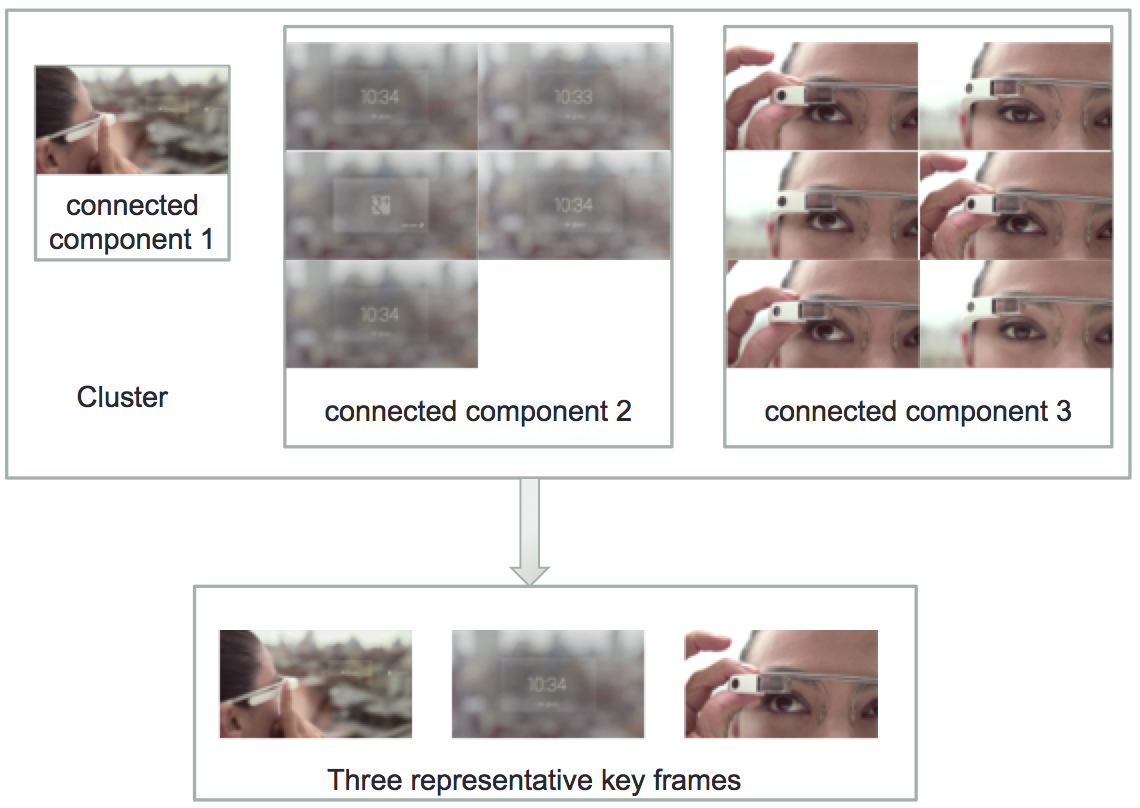
\includegraphics[scale = 0.6]{./keyFrames.png}
  \caption{Key frames identification}
  \end{figure}









